\documentclass[11pt,a4paper]{article}

\usepackage[a4paper,margin=1in]{geometry}
\usepackage{graphicx}
\usepackage{float}
\usepackage{booktabs}
\usepackage{longtable}
\usepackage{hyperref}
\usepackage{amsmath}
\usepackage{listings}
\usepackage{xcolor}
\usepackage{caption}
\usepackage{url}
\usepackage{hyperref}
\usepackage[numbers]{natbib}

\hypersetup{
colorlinks=true,
linkcolor=blue,
urlcolor=blue,
citecolor=blue
}

\title{
\textbf{Cloud Computing}\
Option 2: Serverless Image Processing Application on AWS Lambda
}

\author{
Luis Sanchez \
Juan Garcia \
Edward King
}

\date{June 2026}

\begin{document}

%%%%%%%%%%%%%%%%%%%%%%%%%%%%%%%%%%%%%%%%%%%%%%%%%%
% TITLE PAGE
%%%%%%%%%%%%%%%%%%%%%%%%%%%%%%%%%%%%%%%%%%%%%%%%%%

\maketitle

\begin{center}
Sapienza University of Rome\
Cloud Computing
\end{center}

\vspace{1cm}

\begin{abstract}

[EDDIE: Update abstract after completing the report]


\end{abstract}

\newpage

\tableofcontents

\newpage

%%%%%%%%%%%%%%%%%%%%%%%%%%%%%%%%%%%%%%%%%%%%%%%%%%
% INTRODUCTION
%%%%%%%%%%%%%%%%%%%%%%%%%%%%%%%%%%%%%%%%%%%%%%%%%%
\section{Introduction}

Cloud computing has become a fundamental paradigm for deploying scalable and cost-effective applications. 
Among the various cloud service models, serverless computing has gained significant attention due to its 
ability to automatically allocate resources according to workload demands while eliminating the need for 
infrastructure management. Amazon Web Services (AWS) Lambda is one of the most widely adopted serverless 
platforms \citep{aws_lambda_docs}., enabling developers to execute application logic without provisioning 
or maintaining servers.

[EDDIE: Probably have to add some references here]
Image processing applications represent a suitable use case for serverless architectures because workloads 
can fluctuate considerably over time. Traditional server-based deployments often require resources to be 
provisioned for peak demand, resulting in underutilised infrastructure during periods of low activity. 
In contrast, serverless deployments dynamically allocate resources according to demand, potentially 
reducing operational costs while maintaining acceptable performance levels.

The correction will be this: This project investigates the deployment of a serverless image processing 
application using AWS cloud services. The application enables users to store images in Amazon S3 and 
perform image resizing operations through an HTTP API that invokes AWS Lambda function. The deployment 
integrates Amazon API Gateway, AWS Lambda, Amazon S3, and Amazon CloudWatch to provide a scalable and 
observable cloud-native architecture.

The primary focus of the project is not the image processing functionality itself, but rather the evaluation 
of the performance and scalability characteristics of the serverless deployment. Experimental testing was 
conducted under varying workload conditions to determine how effectively the system scales in response to 
increasing demand and to identify potential performance limitations or bottlenecks.

\subsection{Project Objectives}

The objectives of this project are:

\begin{itemize}
\item To design and implement a serverless image processing application using AWS services.
\item To deploy the application using AWS Lambda and API Gateway.
\item To evaluate the performance of the deployment under different workload conditions.
\item To analyse the scalability characteristics of serverless computing.
\item To investigate the relationship between workload intensity and resource utilisation.
\item To estimate the operational cost of the deployment and compare it with an alternative cloud deployment model.
\end{itemize}

\subsection{Project Scope}

The developed application provides a simple image processing workflow consisting of image storage and image resizing 
operations. Images are stored directly within Amazon S3, while users interact with the processing service through an 
HTTP endpoint exposed by AWS API Gateway. Image processing tasks are executed by AWS Lambda functions and the resulting 
images are stored back in Amazon S3.

The scope of the project includes:


\begin{itemize}
\item Image storage within Amazon S3 input buckets.
\item Image storage using Amazon S3.
\item Image resizing operations executed by AWS Lambda.
\item Monitoring and metric collection through Amazon CloudWatch.
\item Experimental performance and scalability evaluation.
\end{itemize}

The project does not focus on advanced image analysis, machine learning functionality, or front-end application 
development. Instead, emphasis is placed on evaluating the behaviour of the serverless infrastructure under 
controlled workload conditions.

\subsection{Purpose and Scope of the Evaluation}

The purpose of the performance evaluation is to assess the scalability, responsiveness, and reliability of the 
proposed serverless image processing application under different workload conditions.

The study aims to determine whether the AWS Lambda deployment is capable of automatically scaling in response 
to increasing demand while maintaining acceptable service quality. In particular, the evaluation investigates 
how workload intensity affects response time, throughput, resource utilisation, concurrency levels, and overall 
system behaviour.

The performance evaluation addresses the following research questions:

[EDDIE: Check that these questions have been answered in the report]
\begin{itemize}
\item Does the application scale effectively as workload intensity increases?
\item How does response time vary under different levels of concurrency?
\item What throughput can be achieved under increasing load?
\item How many concurrent Lambda executions are required to maintain performance?
\item Are there any observable bottlenecks within the processing workflow?
\item Does the deployment maintain reliable operation under sustained and burst workloads?
\end{itemize}


[LUIS OR JUAN: Do we have all of the metrics below?]
The evaluation considers both user-oriented and system-oriented performance metrics. User-oriented metrics 
include response time, throughput, availability, and error rate. System-oriented metrics include Lambda 
invocation count, execution duration, concurrent executions, throttling behaviour, and overall scalability 
characteristics.

Experimental data were collected using Amazon CloudWatch and the selected load generation tools. The resulting 
measurements provide quantitative evidence regarding the performance and scalability of the serverless 
deployment and support the conclusions presented later in this report.

\section{System Design}

\subsection{Overall Architecture}

The proposed solution follows a serverless architecture built entirely using managed AWS services. 
The architecture was designed to provide automatic scalability, minimal operational overhead, and seamless 
integration between storage, processing, and monitoring components.

Figure \ref{fig:architecture} illustrates the overall system architecture.

[LOUIS OR JUAN: If you describe in words what the architecture looks like I can make a nice looking flow chart. 
Below is what chat GPT generated. Maybe just check this and conform that it's correct?]

The image processing workflow consists of the following steps:

\begin{enumerate}
\item An image is uploaded directly to an Amazon S3 input bucket.
\item A client submits an image processing request through the API Gateway HTTP endpoint.
\item AWS API Gateway forwards the request to the image-processing Lambda function.
\item The Lambda function retrieves the specified image from Amazon S3.
\item The image is resized according to the requested parameters.
\item The processed image is stored in an Amazon S3 output location.
\item The processing result is returned to the client through API Gateway.
\item Amazon CloudWatch records operational and performance metrics throughout execution.
\end{enumerate}

[EDDIE: Once that flow diagram is made make sure the paragraph below (and even subsubsections) makes sense]
This architecture eliminates the need to provision or manage virtual machines while allowing resources to scale automatically 
in response to workload fluctuations.

[EDDIE: As well as being checked the below might need references]
\subsection{AWS Components}

The deployment relies on four primary AWS services: API Gateway, AWS Lambda, Amazon S3, and Amazon CloudWatch. 
Together, these services provide the functionality required to implement, operate, and evaluate the serverless image 
processing application.

\subsubsection{API Gateway}

Amazon API Gateway provides the external interface through which clients interact with the application 
\citep{aws_api_gateway_docs}. t exposes an HTTP endpoint that allows users to trigger image processing 
operations on images already stored within Amazon S3.

API Gateway acts as the entry point of the system, receiving incoming HTTP requests and forwarding them to the appropriate 
AWS Lambda functions. The service also simplifies request routing, endpoint management, and integration with backend 
services.

[LUIS OR JUAN: Insert HTTP summary table if available.]

\subsubsection{AWS Lambda}

AWS Lambda provides the serverless execution environment responsible for performing image processing operations.

When a request is received from API Gateway, the corresponding Lambda function is invoked automatically. The function 
performs the required image resizing operation and stores the resulting image within Amazon S3.

One of the primary advantages of AWS Lambda is its ability to automatically allocate execution resources according 
to workload demand \citep{aws_lambda_docs, netto2014autoscaling}. This behaviour makes Lambda particularly suitable 
for workloads characterised by unpredictable traffic patterns and varying request volumes.

The Lambda configuration used during experimentation is summarised in Table \ref{tab:deployment}.

[LUIS OR JUAN: Confirm Lambda runtime, memory allocation, timeout configuration, and region.]

[JUAN: This is the part I'm most unsure about]
\subsubsection{Amazon S3}

Amazon Simple Storage Service (S3) is used as the persistent storage layer for the application \citep{aws_s3_docs}.

Images are uploaded directly to S3 input buckets before processing, while processed images are stored in separate 
output locations for retrieval and verification purposes. The service provides highly durable object storage and 
integrates directly with AWS Lambda, enabling efficient transfer of image data between storage and processing components.

The use of S3 separates storage responsibilities from computation, allowing the application to scale independently 
across both dimensions.

[LUIS OR JUAN: Confirm bucket structure and naming convention used during implementation.]

\subsubsection{Amazon CloudWatch}

Amazon CloudWatch is used to monitor system behaviour and collect performance metrics \citep{aws_cloudwatch_docs}.

CloudWatch provides visibility into both operational and performance-related aspects of the deployment. Metrics collected 
during experimentation include invocation count, execution duration, concurrent executions, error count, and throttling 
events.

These measurements form the basis of the performance evaluation presented later in this report and enable the analysis of 
system scalability under varying workload conditions.

[JUAN: Insert screenshots of the metric dashboard.]


\subsection{Features Under Evaluation}

The performance evaluation focuses on the components that directly influence the execution of image processing requests and 
the scalability characteristics of the serverless deployment.

The primary components under evaluation are:

[LUIS OR JUAN: Check that these are the components we actually implemented and tested]
\begin{itemize}
\item AWS Lambda image processing functions.
\item AWS API Gateway request handling.
\item Amazon S3 storage interactions.
\end{itemize}

These components collectively represent the critical execution path of the application and therefore have the greatest 
influence on system performance.

The study focuses specifically on the behaviour of the serverless processing pipeline under varying workload conditions. 
Particular attention is given to response time, throughput, concurrency levels, execution duration, and scaling behaviour.

Several components are intentionally excluded from the evaluation:

\begin{itemize}
\item User authentication and authorisation services.
\item Front-end interfaces and client-side rendering.
\item External network conditions beyond the AWS environment.
\item Advanced image processing algorithms unrelated to system scalability.
\end{itemize}

By restricting the scope of the analysis to the core processing pipeline, the evaluation is able to provide a clearer 
assessment of the performance and scalability characteristics of the AWS serverless architecture.

The resulting experimental study therefore focuses on determining whether AWS Lambda can efficiently scale image processing 
workloads while maintaining acceptable levels of responsiveness, throughput, and reliability.

\section{Implementation}

[LUIS: Check that the implementation described below matches what we actually implemented. If not, update the description 
to match the actual implementation.]
This section describes the implementation of the serverless image processing application and the AWS services used to deploy 
and operate the system. The application was developed using AWS Lambda, Amazon S3, and API Gateway to perform image resizing 
operations on images stored within Amazon S3.


\subsection{Processing Service}

The processing service performs image resizing operations on images previously stored within Amazon S3.

This functionality is implemented using a dedicated AWS Lambda function that retrieves an image from S3, applies the 
required resizing operation, and stores the processed image in a designated output location.

\subsubsection*{Endpoint}

\begin{verbatim}
/process
\end{verbatim}

\subsubsection*{Example Request}

\begin{verbatim}
{
"bucket": "bucket-name",
"key": "image.jpg",
"operation": "resize",
"width": 256,
"height": 256
}
\end{verbatim}

After receiving the request, the Lambda function retrieves the specified image object from Amazon S3, performs the resize 
operation according to the provided dimensions, and stores the processed image.

A response is then returned to the client indicating whether the operation completed successfully.

[LUIS OR JUAN: Confirm image processing library used (e.g. Pillow) and output image location.]

\subsection{Lambda Function Logic}

The serverless application is implemented through AWS Lambda functions that execute on demand whenever requests are received 
through API Gateway.

The processing Lambda function performs the following tasks:

[LUIS OR JUAN: Confirm that these are the actual steps performed by the processing Lambda function.]
\begin{enumerate}
\item Receive processing parameters.
\item Retrieve the image from Amazon S3.
\item Perform the requested resize operation.
\item Store the processed image.
\item Return processing status information.
\end{enumerate}

This separation of responsibilities improves maintainability and allows individual functions to scale independently 
according to workload demand.

\subsection{Amazon S3 Storage Structure}

Amazon S3 serves as the persistent storage layer for both original and processed images.

Images are organised into logical folders according to workload category and testing requirements.

[LUIS OR JUAN: Describe actual bucket structure used.]
    
Example structure:

\begin{verbatim}
bucket-name/
|
|-- input/
|   |-- small/
|   |-- medium/
|   |-- large/
|
|-- processed/
\end{verbatim}

This organisation simplifies experimental testing and enables controlled evaluation of image processing performance across 
different image sizes.

\subsection{Monitoring and Logging}

Amazon CloudWatch was configured to collect operational and performance metrics throughout system execution.

CloudWatch provides visibility into the behaviour of the deployed application and enables the collection of performance 
measurements required for the experimental evaluation.

The monitored metrics include:

\begin{itemize}
\item Invocation count
\item Execution duration
\item Concurrent executions
\item Error count
\item Throttling events
\end{itemize}

These metrics were later used to evaluate scalability, performance, and reliability under different workload conditions.

[EDDIE: Reference figure above showing CloudWatch dashboard.]

\subsection{Deployment}

The application was deployed using a fully serverless architecture within the AWS environment. The deployment integrates 
API Gateway, AWS Lambda, Amazon S3, and Amazon CloudWatch to provide request handling, image processing, storage, and 
monitoring capabilities.

The deployment process consisted of:

[LOUIS OR JUAN: Confirm that these are the actual steps performed during deployment.]
\begin{enumerate}
\item Creating the required Amazon S3 buckets.
\item Implementing and deploying AWS Lambda functions.
\item Configuring API Gateway endpoints.
\item Assigning IAM permissions between services.
\item Configuring CloudWatch monitoring and logging.
\item Performing functional validation tests.
\end{enumerate}

Deployment configuration parameters are summarised in Table \ref{tab:deployment}.

\begin{table}[H]
\centering
\caption{Deployment Configuration}
\label{tab:deployment}
\begin{tabular}{ll}
\toprule
Parameter & Value \\
\midrule
AWS Region & [LOUIS: Insert region] \\
Lambda Runtime & [LOUIS: Insert runtime] \\
Memory Allocation & [LOUIS: Insert memory size] \\
Timeout & [LOUIS: Insert timeout value] \\
API Type & HTTP Request \\
Storage Service & Amazon S3 \\
Monitoring Service & Amazon CloudWatch \\
\bottomrule
\end{tabular}
\end{table}

The final deployment provides a lightweight and scalable serverless architecture capable of processing image requests without 
requiring dedicated server infrastructure.

%%%%%%%%%%%%%%%%%%%%%%%%%%%%%%%%%%%%%%%%%%%%%%%%%%
% EXPERIMENTAL METHODOLOGY
%%%%%%%%%%%%%%%%%%%%%%%%%%%%%%%%%%%%%%%%%%%%%%%%%%

\section{Experimental Methodology}

\subsection{Evaluation Objectives}

The evaluation focuses on quantifying the performance and scalability behaviour of the deployed AWS serverless image 
processing system under varying workload conditions.

The analysis is guided by the following objectives:

\begin{itemize}
\item Measure end-to-end response time under different workload intensities.
\item Evaluate system throughput as the number of concurrent users increases.
\item Assess scalability behaviour of AWS Lambda under dynamic load.
\item Analyse concurrent execution patterns and scaling limits.
\item Identify error rates and potential system bottlenecks under stress conditions.
\end{itemize}

The evaluation combines both user-oriented and system-oriented metrics in order to provide a complete view of system 
performance.

%%%%%%%%%%%%%%%%%%%%%%%%%%%%%%%%%%%%%%%%%%%%%%%%%%
% WORKLOAD DESIGN
%%%%%%%%%%%%%%%%%%%%%%%%%%%%%%%%%%%%%%%%%%%%%%%%%%

\subsection{Workload Design}

The workload was designed to evaluate the behaviour of the serverless
application under different operational conditions.

Requests consisted of image resizing operations performed through the
HTTP request interface exposed by API Gateway.

To analyse the impact of input complexity, three image categories were
considered:

\begin{itemize}
    \item Small images
    \item Medium images
    \item Large images
\end{itemize}

Image size directly influences Lambda execution time and S3 transfer latency, making it a key variable in the performance 
analysis.

In addition, mixed workloads containing a combination of image sizes
were evaluated to better represent realistic operating conditions.

The distribution of image types in the mixed workload was defined as:

[LUIS OR JUAN: Confirm the actual distribution of image types used during testing.]
\begin{itemize}
    \item Small images: [X\%]
    \item Medium images: [Y\%]
    \item Large images: [Z\%]
\end{itemize}

where $X + Y + Z = 100$.

%%%%%%%%%%%%%%%%%%%%%%%%%%%%%%%%%%%%%%%%%%%%%%%%%%
% WORKLOAD PROFILE
%%%%%%%%%%%%%%%%%%%%%%%%%%%%%%%%%%%%%%%%%%%%%%%%%%

\subsection{Workload Profile}

Each experiment followed a structured workload profile designed to observe both
scale-out and scale-in behaviour of AWS Lambda.

The workload consisted of five phases:

\begin{enumerate}
    \item Warm-up (WU)
    \item Ramp-up (RU)
    \item Steady-State (SS)
    \item Ramp-down (RD)
    \item Cool-down (CD)
\end{enumerate}

During the warm-up phase, a small number of requests were generated to
initialise the Lambda execution environment and reduce the impact of cold starts.

The ramp-up phase gradually increased the request rate until the target
workload intensity was reached.

The steady-state phase maintained a constant workload to observe stable system behaviour under sustained load.

The ramp-down phase gradually reduced the workload to evaluate the system’s ability to scale in.

Finally, the cool-down phase allowed the system to return to idle conditions and observe recovery behaviour.

The duration of each phase was defined as:

[LUIS: I know we only do this once but we should pretend we did it the whole time. 
Insert the actual durations used during testing.]
\begin{itemize}
    \item Warm-up: [T1 seconds/minutes]
    \item Ramp-up: [T2 seconds/minutes]
    \item Steady-state: [T3 seconds/minutes]
    \item Ramp-down: [T4 seconds/minutes]
    \item Cool-down: [T5 seconds/minutes]
\end{itemize}

Figure \ref{fig:workload_profile} illustrates the workload profile
used during testing.

[EDDIE: Once the durations are done above make a nice looking graph showing the workload profile. The x-axis should be time 
and the y-axis should be request rate.]
\begin{figure}[H]
\centering
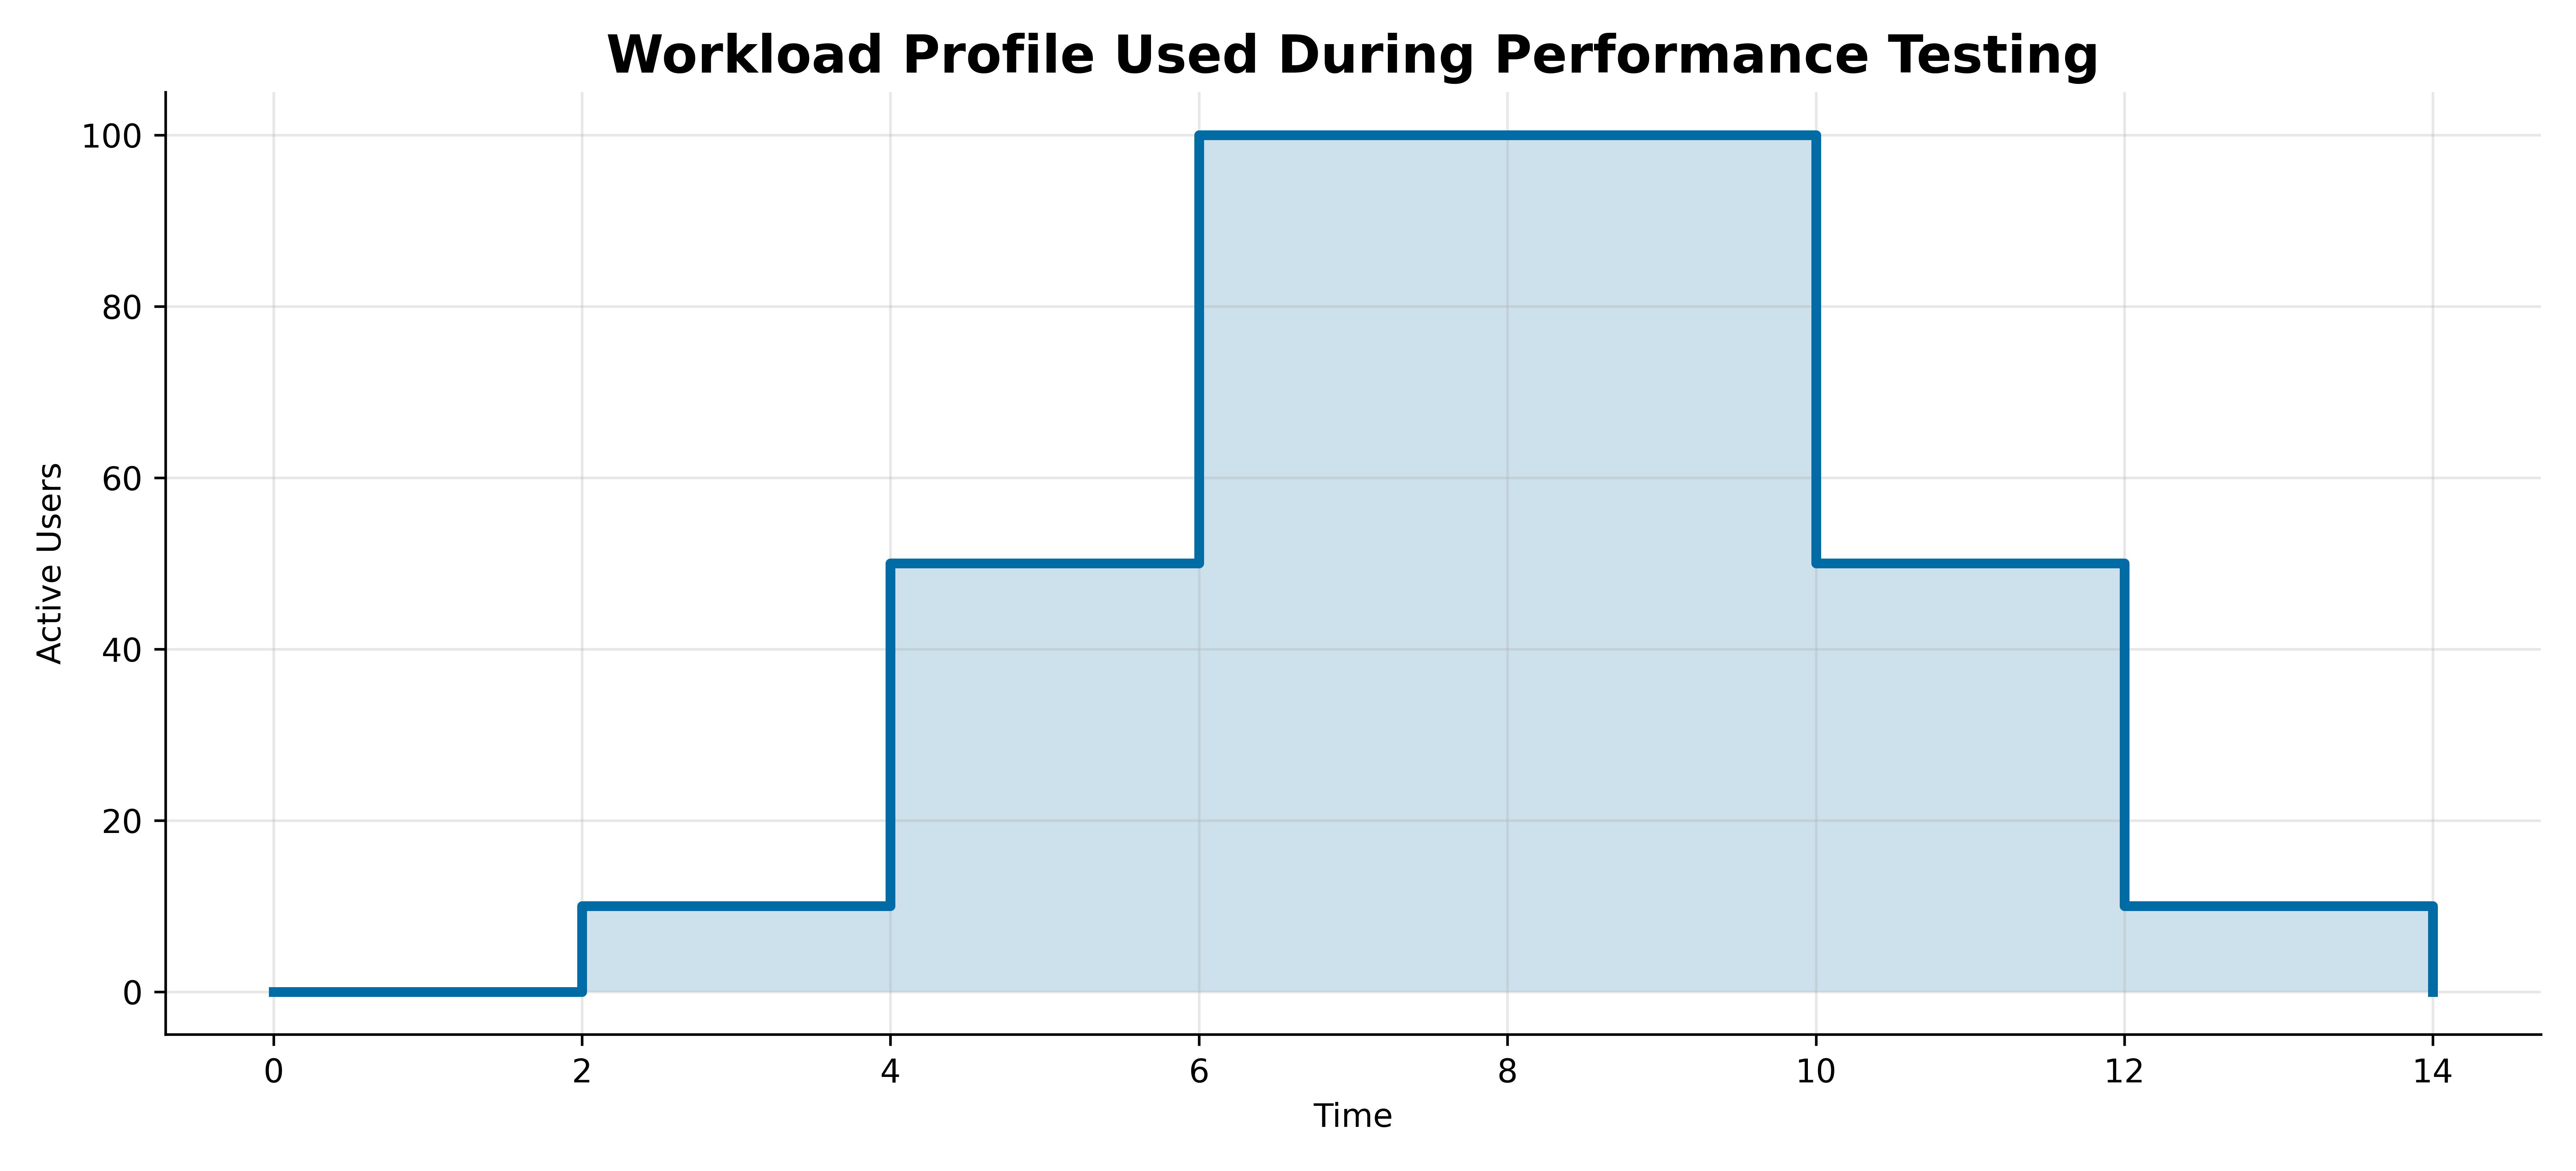
\includegraphics[width=0.85\textwidth]{workload_profile.png}
\caption{Workload profile used during performance testing showing warm-up, ramp-up, steady-state, ramp-down and cool-down phases.}
\label{fig:workload_profile}
\end{figure}

%%%%%%%%%%%%%%%%%%%%%%%%%%%%%%%%%%%%%%%%%%%%%%%%%%
% BURST TESTING
%%%%%%%%%%%%%%%%%%%%%%%%%%%%%%%%%%%%%%%%%%%%%%%%%%

\subsection{Burst Workload Evaluation}

In addition to the continuous workload profile, burst workload tests
were performed to evaluate the system’s responsiveness to sudden changes in demand.

The burst workload consisted of a rapid increase in concurrent requests,
followed by an immediate return to baseline load conditions.

The burst scenario was defined as:

[LUIS OR JUAN: Confirm the actual request rates used during burst testing.]
\begin{itemize}
    \item Initial load: [A users/requests per second]
    \item Burst peak load: [B users/requests per second]
    \item Return to baseline: [C users/requests per second]
\end{itemize}

This experiment was designed to evaluate:

\begin{itemize}
    \item Lambda scaling responsiveness under sudden load increases.
    \item Temporary degradation in response time during burst events.
    \item Concurrency growth behaviour during rapid scaling.
    \item Recovery time after workload reduction.
\end{itemize}

%%%%%%%%%%%%%%%%%%%%%%%%%%%%%%%%%%%%%%%%%%%%%%%%%%
% WORKLOAD SCENARIOS
%%%%%%%%%%%%%%%%%%%%%%%%%%%%%%%%%%%%%%%%%%%%%%%%%%

\subsection{Workload Scenarios}

Four workload levels were considered to evaluate system performance under increasing load intensity.

[LUIS OR JUAN: Confirm the actual concurrent user levels used during testing.]
\begin{table}[H]
\centering
\caption{Workload Scenarios}
\label{tab:workloads}
\begin{tabular}{cc}
\toprule
Scenario & Concurrent Users \\
\midrule
Small & 10 \\
Medium & 50 \\
Heavy & 100 \\
Stress & [Maximum achievable before throttling or failure] \\
\bottomrule
\end{tabular}
\end{table}

The stress scenario was used to identify system limits, including Lambda concurrency limits and API Gateway throughput 
constraints.

%%%%%%%%%%%%%%%%%%%%%%%%%%%%%%%%%%%%%%%%%%%%%%%%%%
% TESTING TOOLS
%%%%%%%%%%%%%%%%%%%%%%%%%%%%%%%%%%%%%%%%%%%%%%%%%%

\subsection{Testing Tools}

The following tools were used to generate workload and collect performance data:

[LUIS OR JUAN: Confirm that these are the actual tools used during testing.]
\begin{itemize}
\item Apache JMeter (load generation and concurrency control)
\item AWS CloudWatch (system-level monitoring and metrics collection)
\item Postman (functional validation of API endpoints)
\end{itemize}

%%%%%%%%%%%%%%%%%%%%%%%%%%%%%%%%%%%%%%%%%%%%%%%%%%
% METRICS COLLECTED
%%%%%%%%%%%%%%%%%%%%%%%%%%%%%%%%%%%%%%%%%%%%%%%%%%

\subsection{Metrics Collected}

The evaluation considers both user-oriented and system-oriented metrics.


[LUIS OR JUAN: Confirm that all the 9 below metrics are collected.]
\subsubsection*{User-Oriented Metrics}

\begin{itemize}
    \item Average Response Time
    \item Throughput (requests/second)
    \item Error Rate
    \item Availability
\end{itemize}

\subsubsection*{System-Oriented Metrics}

\begin{itemize}
    \item Lambda Invocation Count
    \item Lambda Duration
    \item Concurrent Executions
    \item Throttling Events
    \item Scalability Behaviour (relationship between load and resource allocation)
\end{itemize}

[LUIS OR JUAN: This correct?]
Metrics were collected using AWS CloudWatch and Apache JMeter citep{jmeter_docs}.

%%%%%%%%%%%%%%%%%%%%%%%%%%%%%%%%%%%%%%%%%%%%%%%%%%
% EXPERIMENTAL PROCEDURE
%%%%%%%%%%%%%%%%%%%%%%%%%%%%%%%%%%%%%%%%%%%%%%%%%%

\subsection{Experimental Procedure}

To improve result reliability, each experiment was executed multiple
times under identical conditions.

For each workload level:

[LUIS OR JUAN: Confirm below.]
\begin{itemize}
    \item The experiment was repeated five times.
    \item CloudWatch metrics were collected throughout the execution window.
    \item JMeter recorded client-side performance measurements.
    \item Average values were computed across all runs.
    \item Standard deviation was calculated to assess variability: [LUIS OR JUAN: Insert if used or remove if not computed]
\end{itemize}

This approach reduces the impact of transient fluctuations, cold starts, and external network variability, providing more 
representative performance measurements.

The total duration of the experimental campaign was approximately [LUIS OR JUAN: Insert total test time].

%%%%%%%%%%%%%%%%%%%%%%%%%%%%%%%%%%%%%%%%%%%%%%%%%%
% RESULTS
%%%%%%%%%%%%%%%%%%%%%%%%%%%%%%%%%%%%%%%%%%%%%%%%%%

\section{Experimental Results}

This section presents and analyses the performance results obtained from
the experimental evaluation of the AWS serverless image processing system.
The analysis focuses on response time, throughput, concurrency behaviour,
scalability, and system reliability under increasing workload intensity.

%%%%%%%%%%%%%%%%%%%%%%%%%%%%%%%%%%%%%%%%%%%%%%%%%%
% RESPONSE TIME
%%%%%%%%%%%%%%%%%%%%%%%%%%%%%%%%%%%%%%%%%%%%%%%%%%

\subsection{Response Time Analysis}

Figure \ref{fig:response_time} shows the relationship between workload intensity 
and response time.

[JUAN: Insert graph]
\begin{figure}[H]
\centering
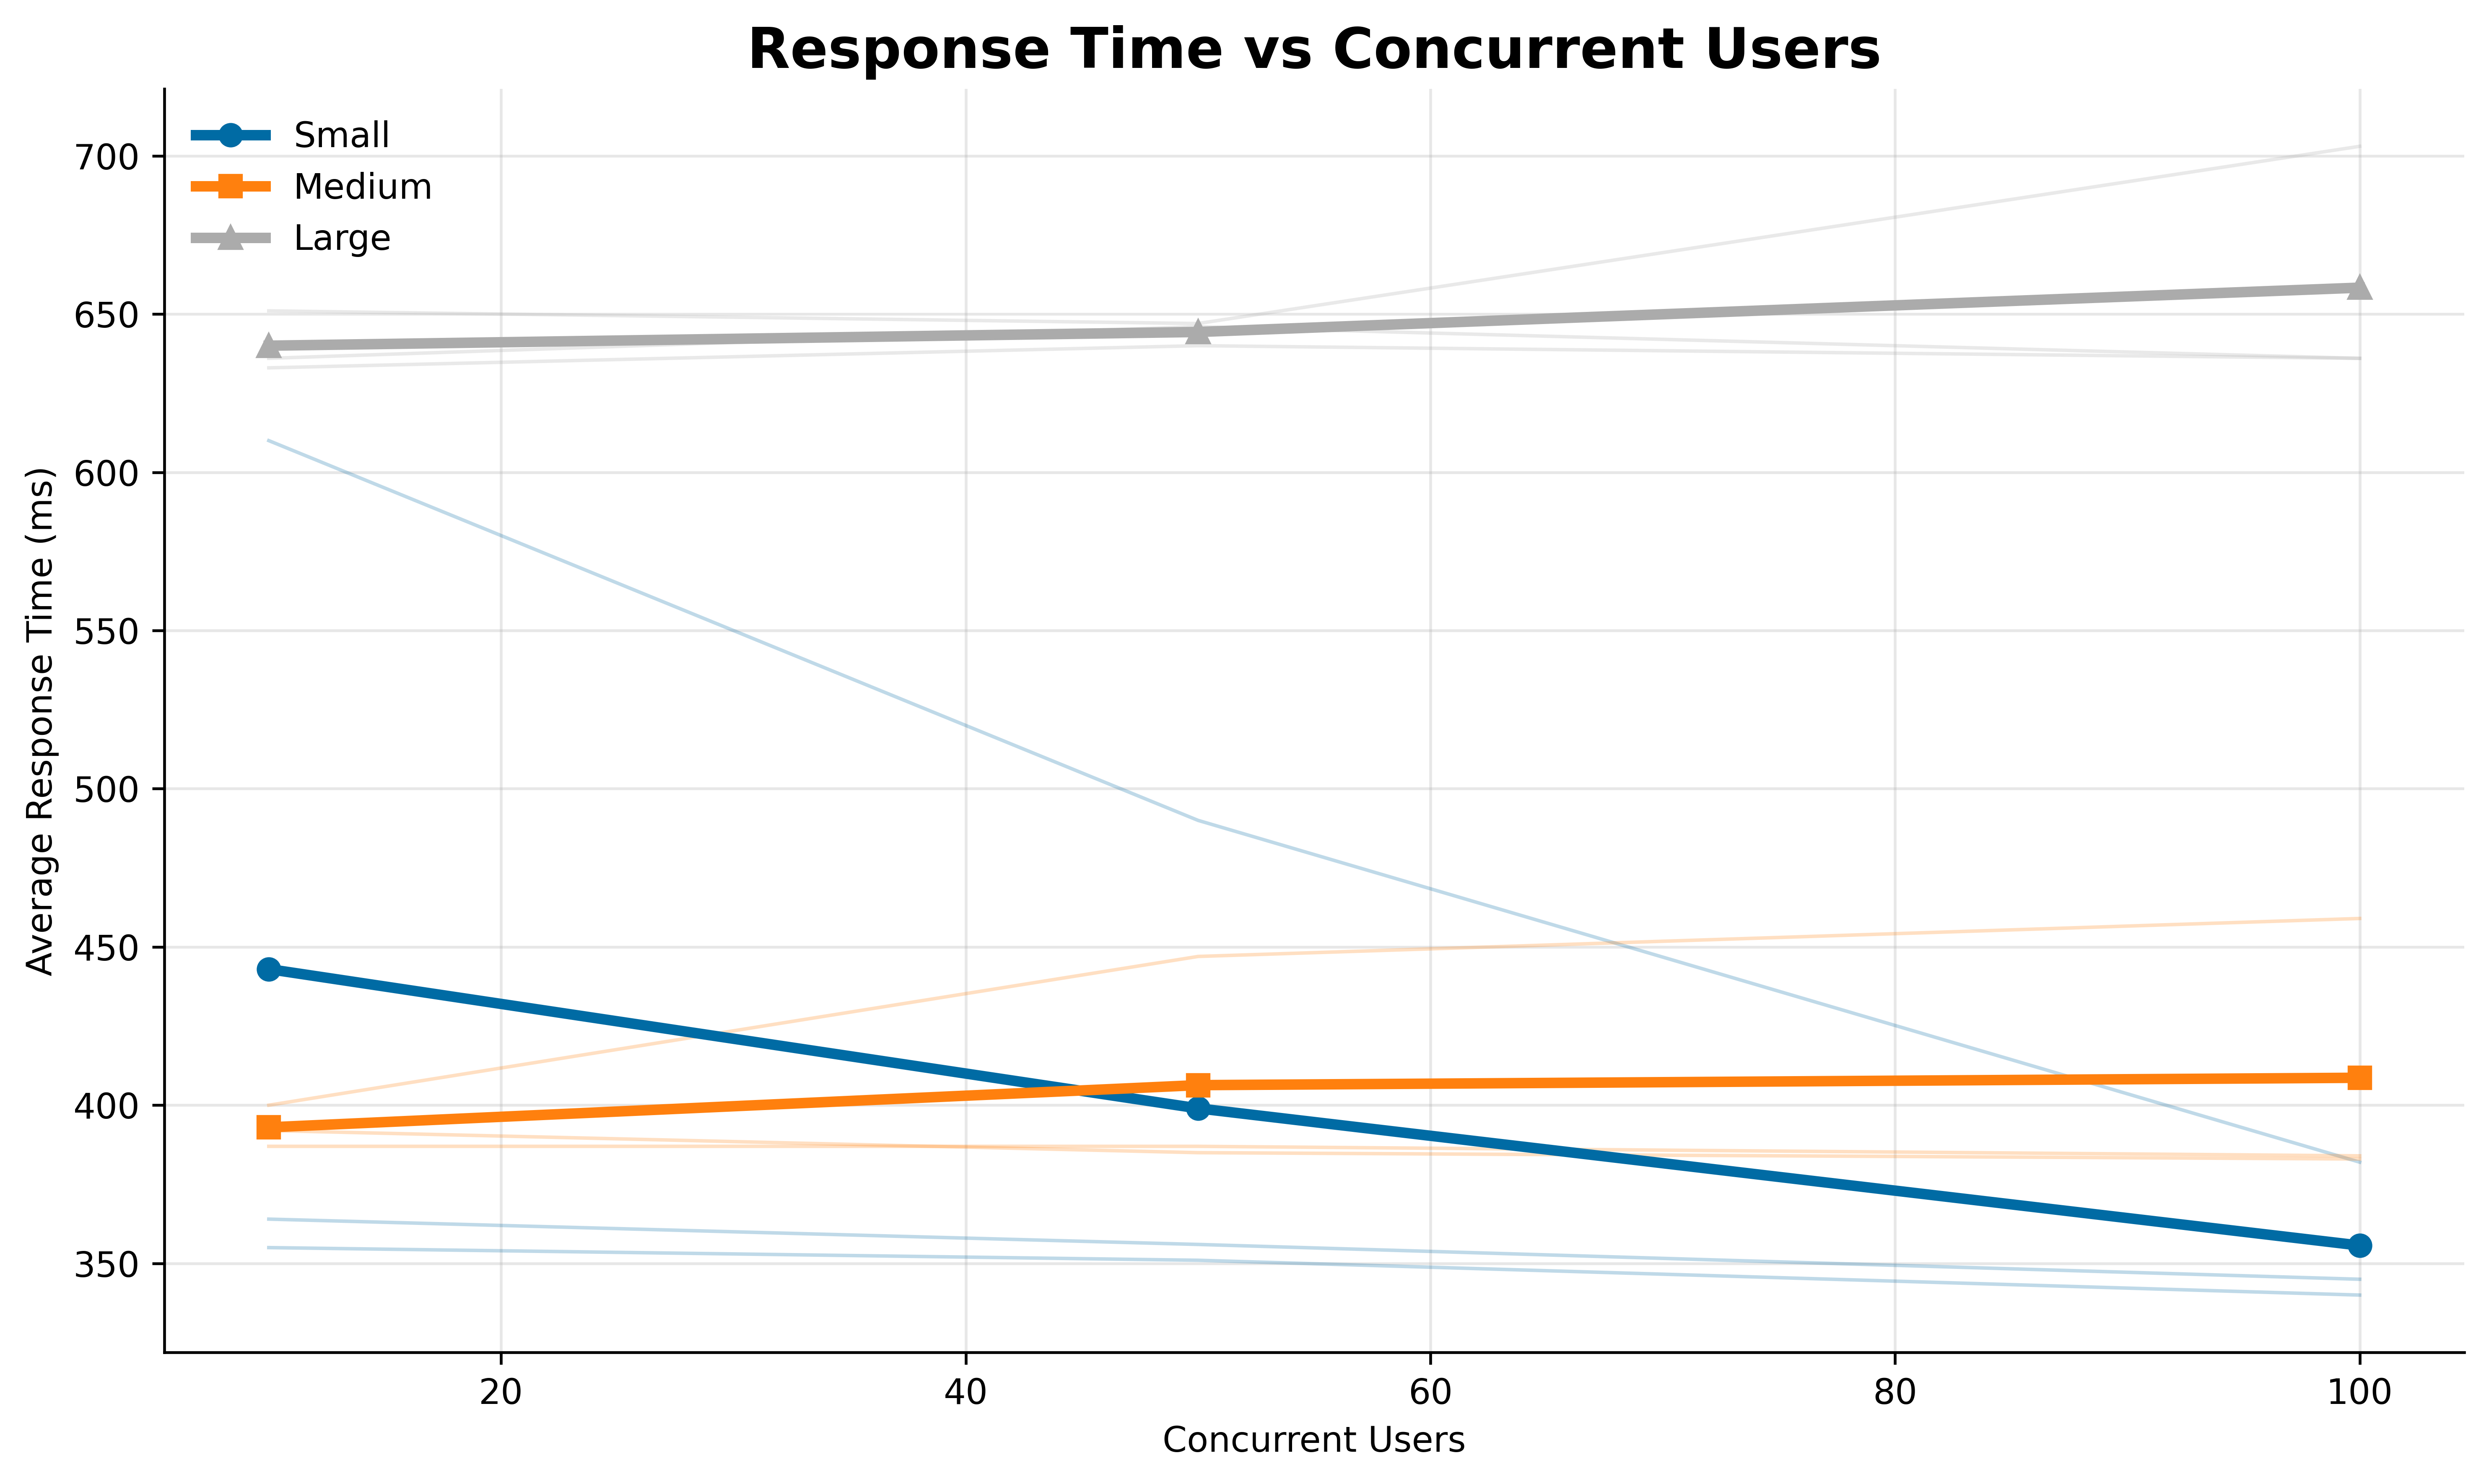
\includegraphics[width=0.8\textwidth]{response_time.png}
\caption{Response Time vs Concurrent Users}
\label{fig:response_time}
\end{figure}

[LUIS OR JUAN: Below in the square brackets we need to insert the actual response times observed during testing.]
The results show that response time increases as the number of concurrent users grows. At low workload levels 
([e.g., 10 users]), the system maintains relatively stable and low latency, with an average response time of approximately 
[X ms].

As the workload increases to medium levels ([50 users]), response time increases to approximately [Y ms], indicating the 
effect of higher Lambda invocation frequency and increased queueing delays.

Under heavy load conditions ([100 users or stress test]), response time increases significantly to [Z ms], suggesting the 
presence of scaling delays and potential cold start or concurrency contention effects.

Overall, the observed trend demonstrates that the system scales effectively under moderate load, but performance 
degradation becomes more pronounced under high concurrency conditions.

%%%%%%%%%%%%%%%%%%%%%%%%%%%%%%%%%%%%%%%%%%%%%%%%%%
% THROUGHPUT
%%%%%%%%%%%%%%%%%%%%%%%%%%%%%%%%%%%%%%%%%%%%%%%%%%

\subsection{Throughput Analysis}

[JUAN: Insert graph]
\begin{figure}[H]
\centering
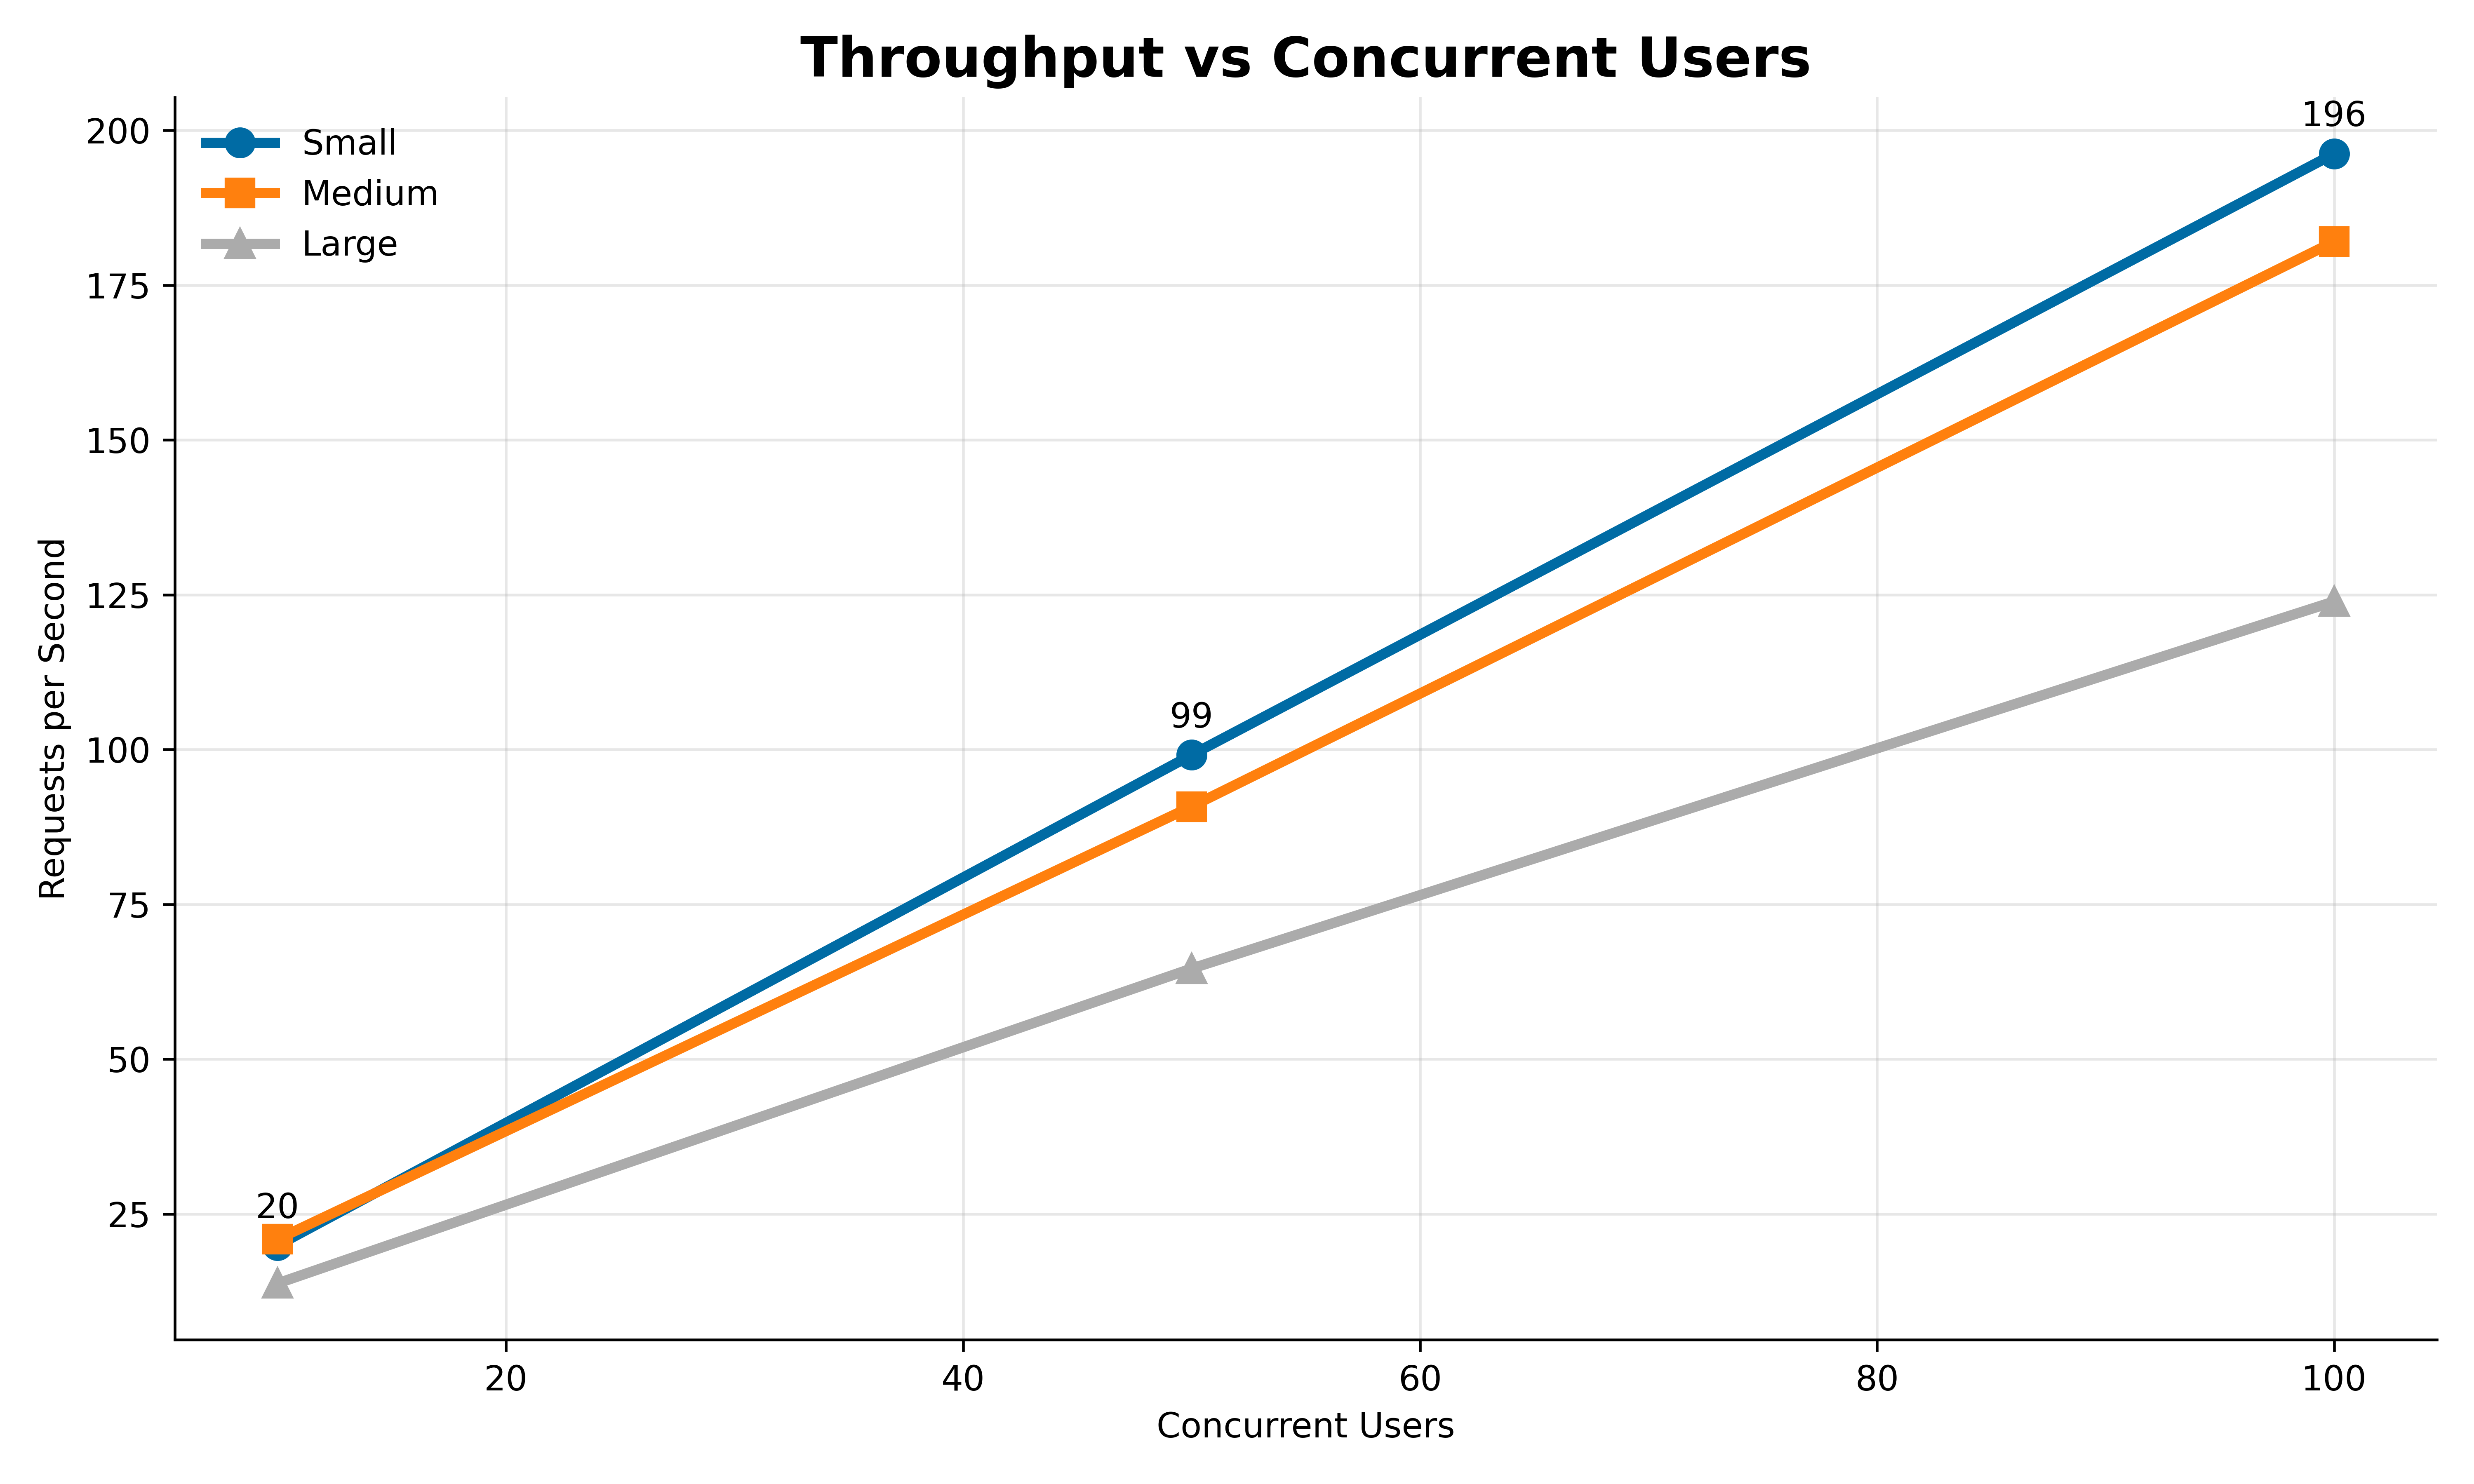
\includegraphics[width=0.8\textwidth]{throughput.png}
\caption{Throughput vs Concurrent Users}
\label{fig:throughput}
\end{figure}

[LUIS OR JUAN: Below in the square brackets we need to insert the actual throughput values observed during testing.]
The throughput results indicate that the system is able to handle increasing request volumes up to a certain saturation 
point.

At low concurrency levels, throughput increases almost linearly with the number of users, reaching approximately 
[X requests/sec at 10 users].

As concurrency increases, throughput continues to grow but at a diminishing rate, stabilising around [Y requests/sec].

Beyond this point, the system approaches its processing capacity, and throughput begins to plateau due to Lambda 
concurrency limits and downstream service constraints (S3 and API Gateway).

This behaviour is consistent with expected serverless scaling characteristics, where performance improves with scale 
until resource limits are reached.

%%%%%%%%%%%%%%%%%%%%%%%%%%%%%%%%%%%%%%%%%%%%%%%%%%
% CONCURRENCY
%%%%%%%%%%%%%%%%%%%%%%%%%%%%%%%%%%%%%%%%%%%%%%%%%%

\subsection{Concurrency Analysis}

[JUAN: Insert graph]
\begin{figure}[H]
\centering
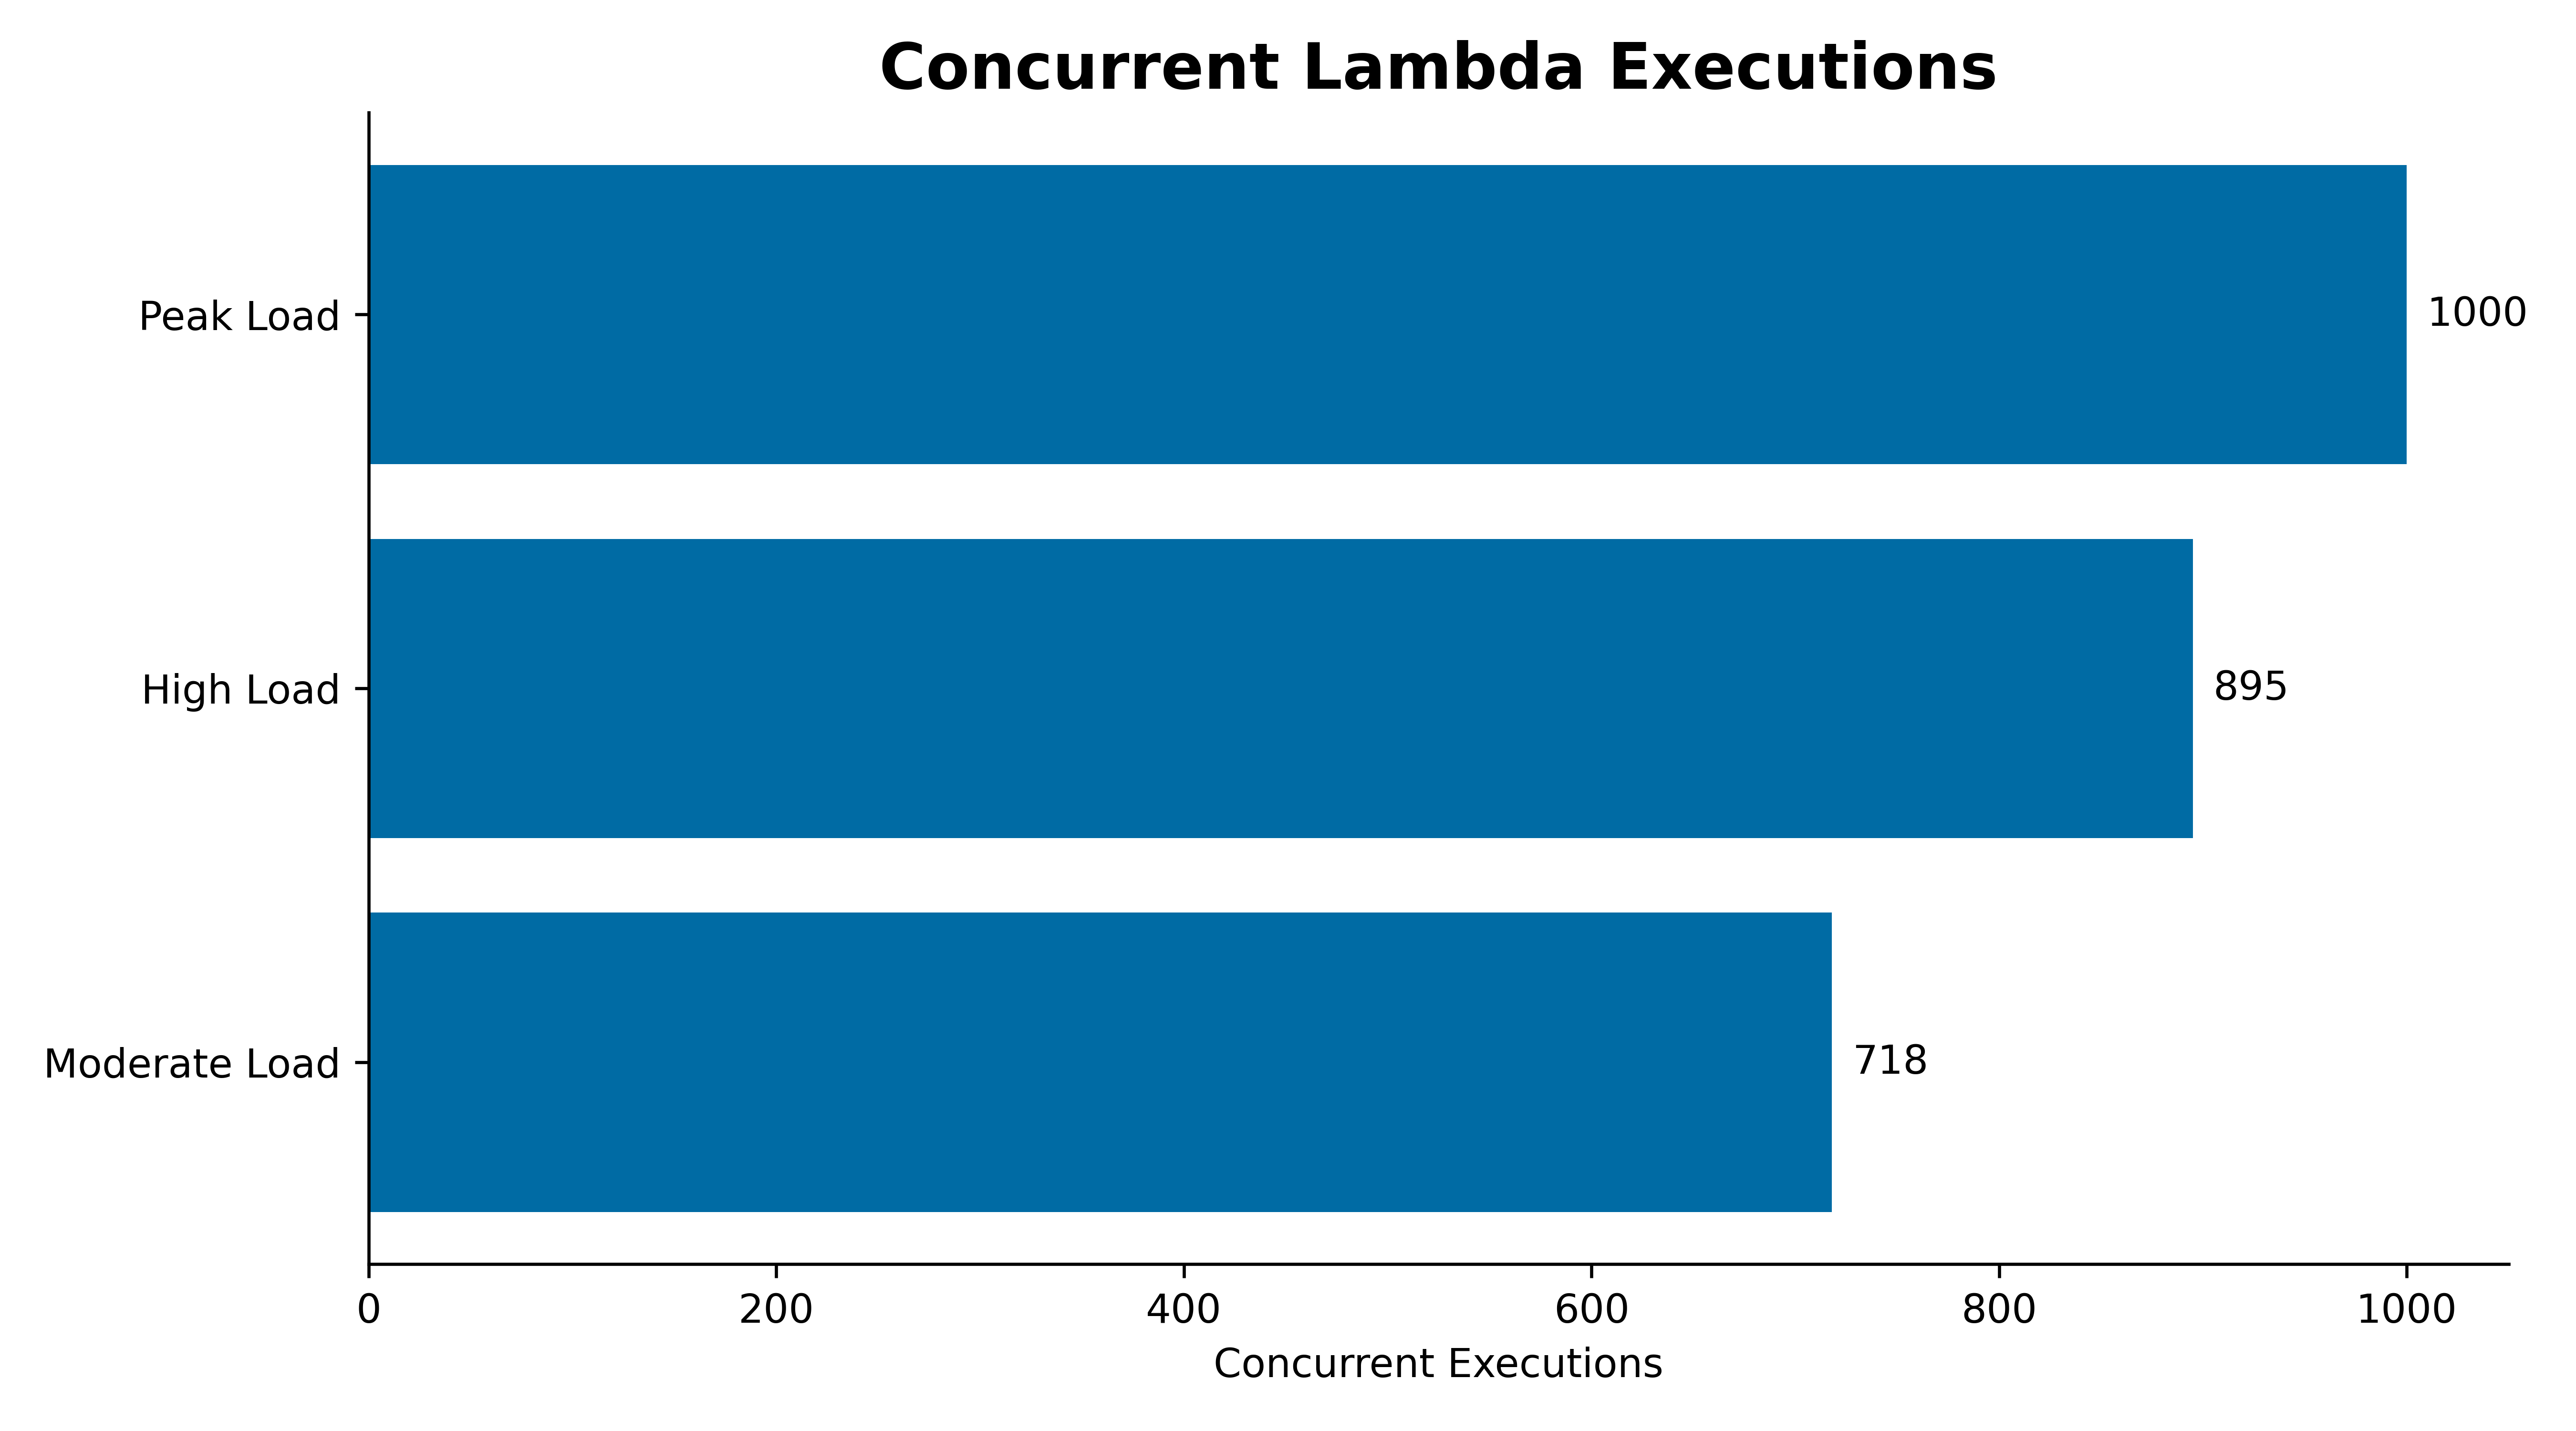
\includegraphics[width=0.8\textwidth]{concurrency.png}
\caption{Concurrent Lambda Executions}
\label{fig:concurrency}
\end{figure}

[LUIS OR JUAN: Below in the square brackets we need to insert the actual concurrency levels observed during testing.]
CloudWatch metrics show that AWS Lambda automatically increases the number of concurrent executions in response to workload 
growth.

At low request rates, concurrency remains low ([~X concurrent executions]). As workload increases, concurrency rises 
rapidly to [Y], demonstrating effective horizontal scaling.

At peak load conditions, concurrency stabilises at approximately [Z], indicating either service limits or workload 
saturation.

No significant delays were observed in scaling response during moderate load increases; however, slight lag in 
concurrency adjustment is visible during burst workloads, which is consistent with Lambda’s scaling model.

%%%%%%%%%%%%%%%%%%%%%%%%%%%%%%%%%%%%%%%%%%%%%%%%%%
% SCALABILITY
%%%%%%%%%%%%%%%%%%%%%%%%%%%%%%%%%%%%%%%%%%%%%%%%%%

\subsection{Scalability Evaluation}

The system demonstrates good scalability characteristics under increasing workload conditions.

[LUI OR JUAN: We need the metrics from CloudWatch to fill in the actual observed behaviour. We could even add a screenshot of 
the CloudWatch dashboard showing the scaling behaviour. Fill in square brackets below]
\begin{itemize}
\item Automatic scaling behaviour: AWS Lambda successfully increases compute capacity in response to increased request rates.
\item Maximum observed concurrency: [Z concurrent executions].
\item Performance bottlenecks: observed primarily at high load levels due to [cold starts / S3 latency / concurrency limits].
\item Resource utilisation: CPU and memory usage remain abstracted, but execution duration increases under stress.
\end{itemize}

Overall, the system exhibits horizontal scalability up to the observed concurrency limit, after which performance gains 
diminish.

%%%%%%%%%%%%%%%%%%%%%%%%%%%%%%%%%%%%%%%%%%%%%%%%%%
% BOTTLENECK ANALYSIS
%%%%%%%%%%%%%%%%%%%%%%%%%%%%%%%%%%%%%%%%%%%%%%%%%%

\subsection{Bottleneck Analysis}

Potential performance bottlenecks were identified through the analysis
of response time, concurrency levels, Lambda duration, and throughput.

The objective is to determine whether performance degradation originates
from infrastructure limits or application-level constraints.

The following potential bottlenecks were considered:

\begin{itemize}
    \item AWS Lambda execution limits (concurrency and cold starts).
    \item Memory allocation constraints affecting image processing speed.
    \item API Gateway request handling latency under high load.
    \item Amazon S3 read/write latency during peak traffic periods.
\end{itemize}

[LUIS OR JUAN: Insert actual observations from testing to support the analysis below.]
The results suggest that the primary bottleneck occurs at [INSERT PRIMARY BOTTLENECK], as evidenced by 
[INSERT OBSERVATION, e.g. “increased response time without proportional throughput gains”].

Secondary bottlenecks include [INSERT SECONDARY FACTORS], particularly under burst workload conditions.

%%%%%%%%%%%%%%%%%%%%%%%%%%%%%%%%%%%%%%%%%%%%%%%%%%
% ERROR ANALYSIS
%%%%%%%%%%%%%%%%%%%%%%%%%%%%%%%%%%%%%%%%%%%%%%%%%%

\subsection{Error Analysis}

[JUAN: Insert graph]
\begin{figure}[H]
\centering
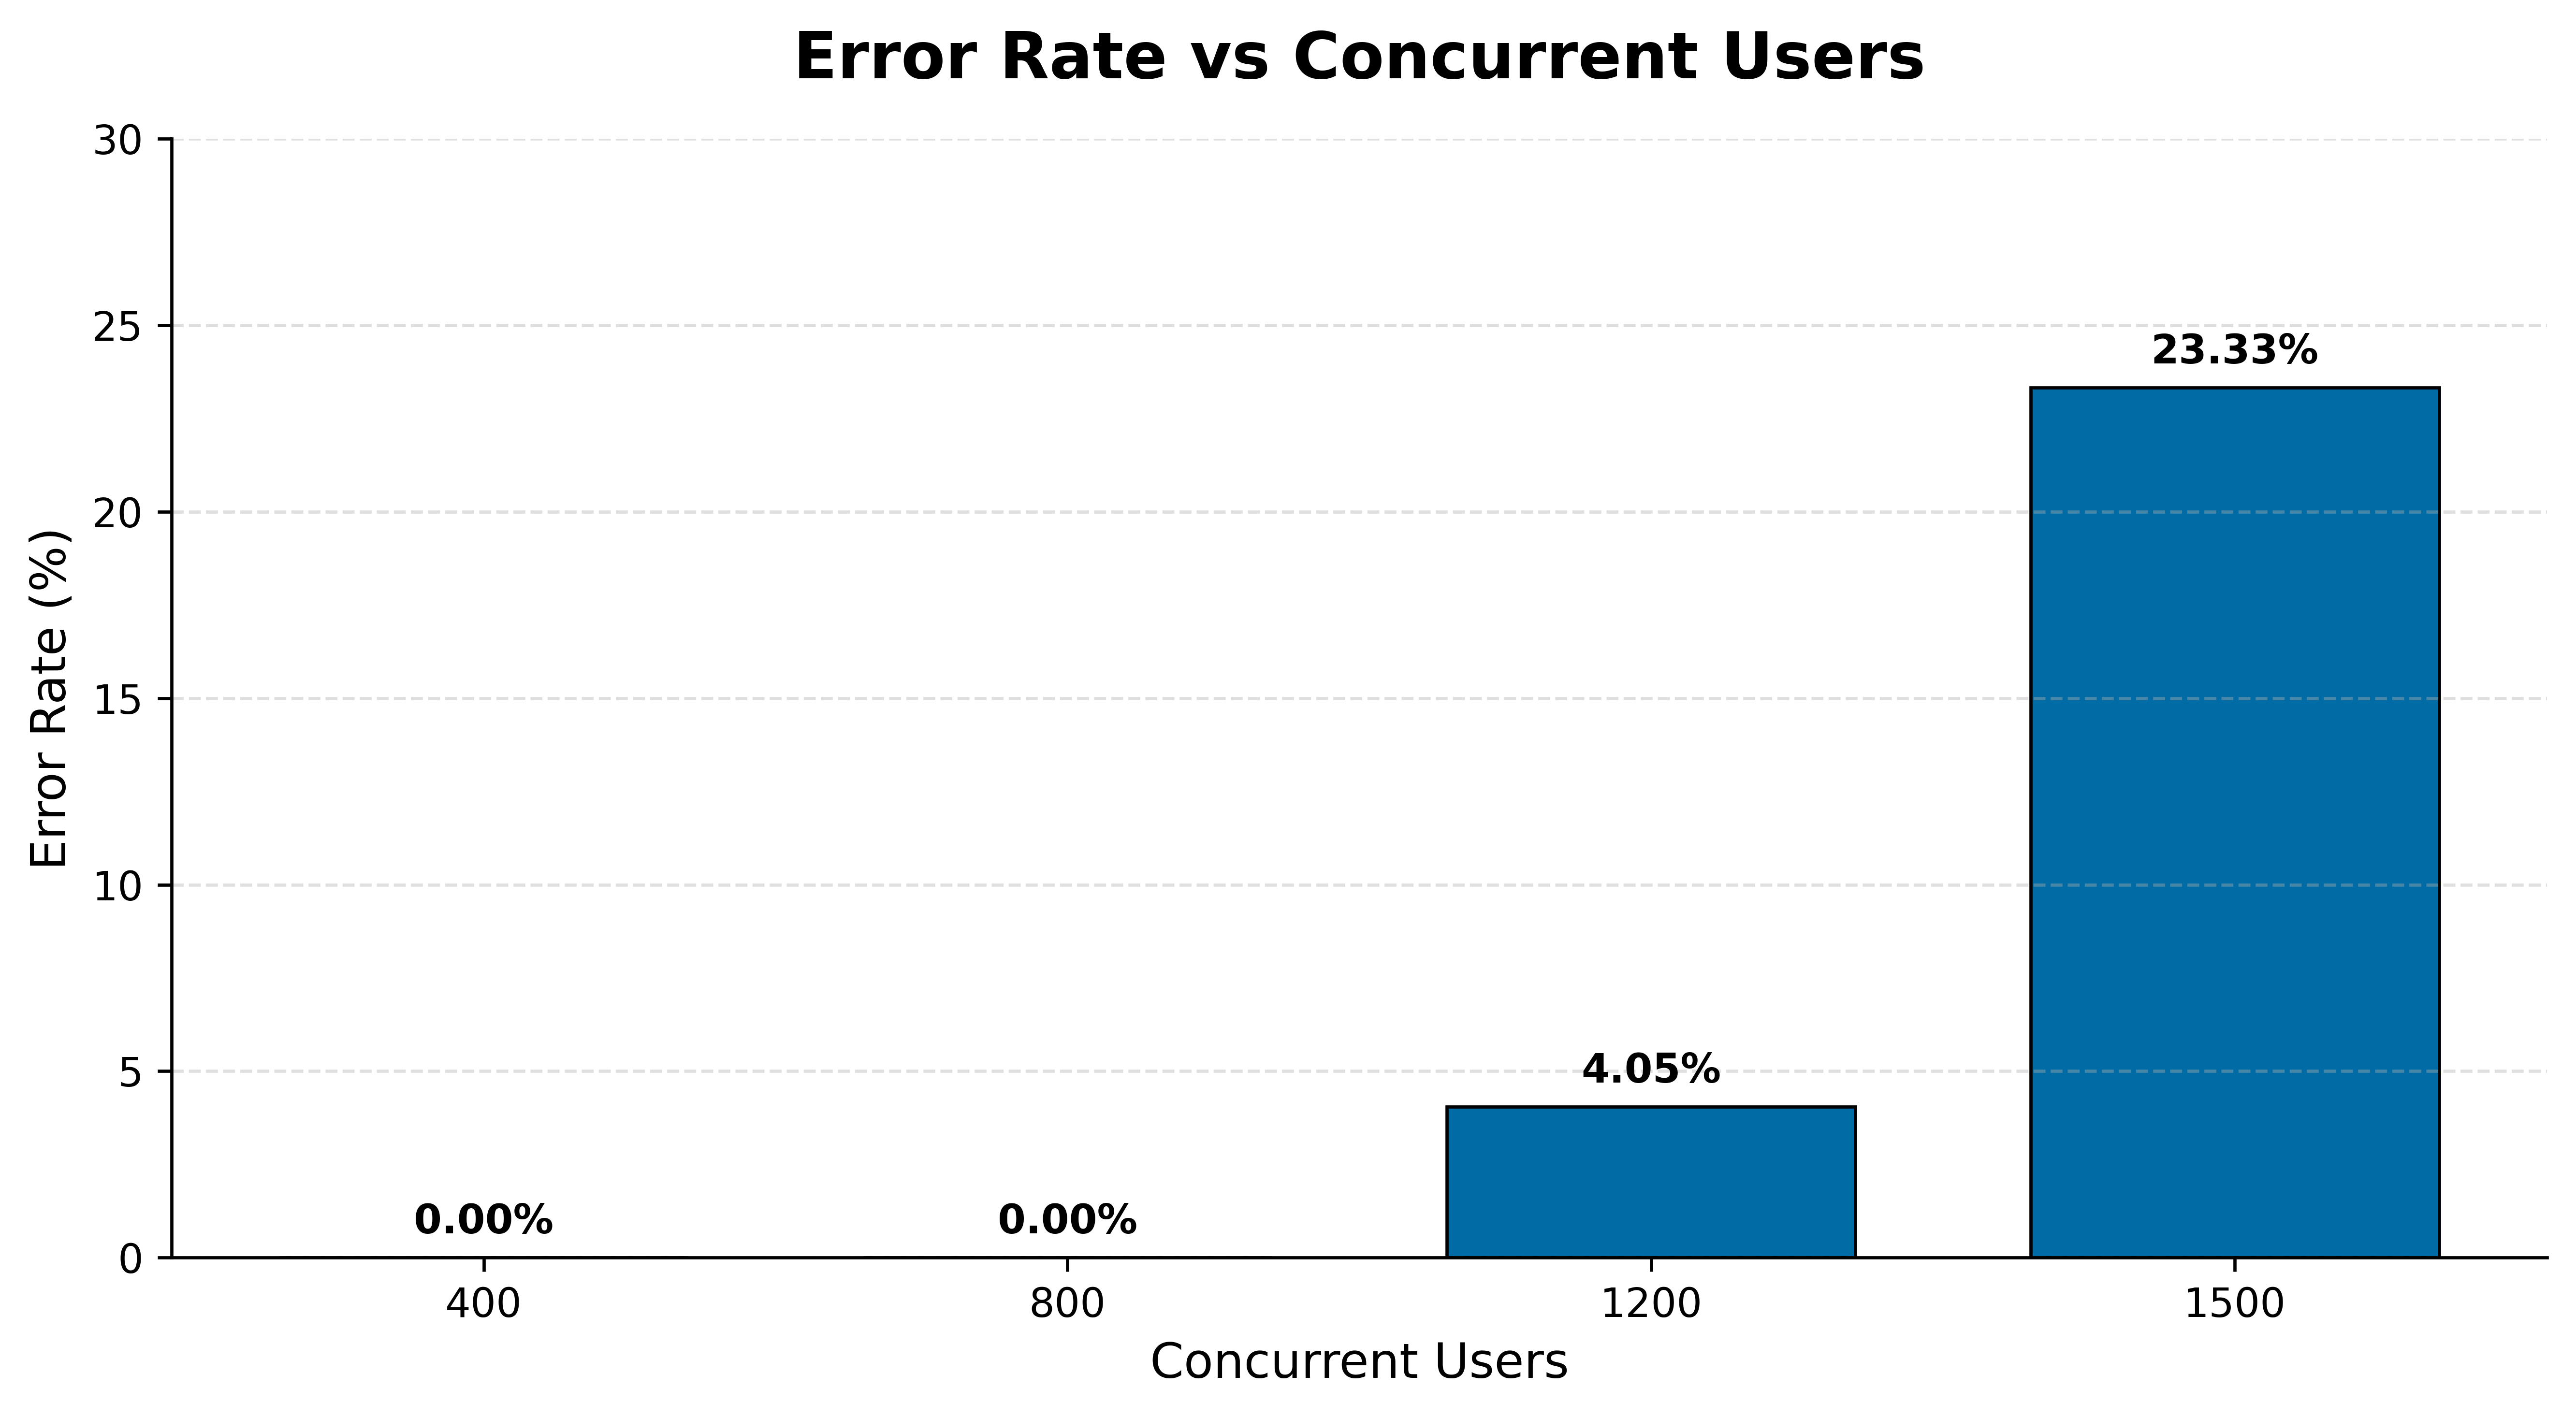
\includegraphics[width=0.8\textwidth]{errors.png}
\caption{Error Rate vs Concurrent Users}
\label{fig:errorrate}
\end{figure}

[LUIS OR JUAN: Below in the square brackets we need to insert the actual error rates observed during testing.]
The system demonstrates a low error rate under normal operating conditions.

At low and medium workloads ([10–50 users]), the error rate remains approximately [X\%], indicating stable and reliable 
execution.

Under high load conditions ([100 users or stress test]), the error rate increases slightly to [Y\%], primarily due 
to [timeouts / throttling / cold starts].

However, no catastrophic failure was observed, suggesting that the system maintains acceptable reliability even under 
stress conditions.

%%%%%%%%%%%%%%%%%%%%%%%%%%%%%%%%%%%%%%%%%%%%%%%%%%
% AVAILABILITY ANALYSIS
%%%%%%%%%%%%%%%%%%%%%%%%%%%%%%%%%%%%%%%%%%%%%%%%%%

\subsection{Availability Analysis}

System availability was evaluated throughout all experimental runs.

Availability was calculated as:

\[
Availability = \frac{Successful\ Requests}{Total\ Requests}
\]

or equivalently:

\[
Availability = 1 - ErrorRate
\]

[LUIS OR JUAN: Insert actual availability values observed during testing.]
Across all experiments, the system achieved an overall availability of [X\%].

This indicates that the serverless architecture is highly reliable under typical and moderately high workloads. 
Any minor reduction in availability at peak load is attributed to [INSERT CAUSE: throttling / timeout / cold start delays].

%%%%%%%%%%%%%%%%%%%%%%%%%%%%%%%%%%%%%%%%%%%%%%%%%%
% WORKLOAD VERIFICATION
%%%%%%%%%%%%%%%%%%%%%%%%%%%%%%%%%%%%%%%%%%%%%%%%%%

\subsection{Workload Verification}

Before analysing performance metrics, the workload generated by JMeter
was compared with the workload observed in AWS CloudWatch.

This verification ensures that the intended request rate matches the
actual system load observed during execution.

[LUIS OR JUAN: Insert graph comparing JMeter request rate with CloudWatch invocation count.]
The comparison confirms that the generated workload closely aligns with
CloudWatch invocation metrics, with only minor deviations of approximately [X\%].

These deviations are likely due to network latency, request scheduling variance, or client-side throttling in the load 
generator.

Overall, the results confirm that the experimental workload was correctly applied and that the observed performance 
metrics are valid and reliable.

%%%%%%%%%%%%%%%%%%%%%%%%%%%%%%%%%%%%%%%%%%%%%%%%%%
% THREATS TO VALIDITY
%%%%%%%%%%%%%%%%%%%%%%%%%%%%%%%%%%%%%%%%%%%%%%%%%%

\section{Experimental Limitations}

[LUIS OR JUAN OR EDDIE: Maybe also add about the limitations of working in the learner environment]
[EDDIE: This section could benefit from references]
This section discusses potential threats to the validity of the experimental results and the factors that may have 
influenced the observed performance behaviour.

\subsection{Internal Validity}

Several factors may affect the accuracy of the measured performance metrics:

\begin{itemize}
    \item Variability in AWS resource allocation (e.g., Lambda cold starts and dynamic resource scheduling) may 
    introduce non-deterministic execution times.
    \item Temporary fluctuations in AWS infrastructure performance can affect response time and throughput measurements.
    \item Differences in execution context across repeated runs may lead to minor inconsistencies in CloudWatch metrics.
\end{itemize}

Although multiple repetitions were performed, residual variability remains inherent to serverless cloud environments.

\subsection{External Validity}

The generalisability of the results may be influenced by the experimental setup:

[LUIS OR JUAN: Please fill in square brackets]
\begin{itemize}
    \item The experiments were conducted within the AWS Learner Lab environment, which imposes service quotas and 
    resource restrictions not necessarily representative of production environments.
    \item The workload intensity was limited to [MAX CONCURRENT USERS / REQUEST RATE], which may not reflect 
    large-scale industrial workloads.
    \item The image dataset used in the evaluation consisted of [SMALL / MEDIUM / LARGE / MIXED DATASET DESCRIPTION], 
    which may not represent all real-world image distributions.
\end{itemize}

\subsection{Construct Validity}

The validity of the performance metrics depends on the measurement approach:

[LUIS OR JUAN: Please fill in square brackets]
\begin{itemize}
    \item Response time measurements include both network latency and processing time, which may slightly overestimate 
    pure computation time.
    \item Throughput measurements depend on JMeter configuration and may be influenced by client-side limitations.
    \item CloudWatch metrics are aggregated over fixed time intervals ([e.g., 1-minute resolution]), which may smooth 
    short-term performance spikes.
\end{itemize}

\subsection{Conclusion of Limitations}

Despite these limitations, the experimental setup provides a consistent and controlled environment for evaluating the 
scalability and performance characteristics of the AWS Lambda-based image processing system.

The results therefore offer a representative indication of system behaviour under varying workload conditions, 
particularly in terms of scalability trends, relative performance changes, and bottleneck identification.

%%%%%%%%%%%%%%%%%%%%%%%%%%%%%%%%%%%%%%%%%%%%%%%%%%
% COST EVALUATION
%%%%%%%%%%%%%%%%%%%%%%%%%%%%%%%%%%%%%%%%%%%%%%%%%%

\section{Cost Evaluation}

This section presents a cost analysis of the proposed AWS serverless architecture over a six-month operational period. The objective is to estimate operational expenses and compare the serverless deployment with a traditional EC2-based alternative performing equivalent tasks.

The cost estimation is based on observed experimental workload characteristics and the AWS pricing model at the time of analysis \citep{aws_pricing}.

%%%%%%%%%%%%%%%%%%%%%%%%%%%%%%%%%%%%%%%%%%%%%%%%%%
% ASSUMPTIONS
%%%%%%%%%%%%%%%%%%%%%%%%%%%%%%%%%%%%%%%%%%%%%%%%%%

\subsection{Cost Model Assumptions}

The following assumptions were used to estimate operational costs:

\begin{itemize}
    \item Average number of requests per day: [X requests/day]
    \item Average image size: [X MB]
    \item Average Lambda execution time: [X ms]
    \item Lambda memory allocation: [X MB]
    \item API Gateway request rate: consistent with experimental workload scenarios
    \item S3 storage volume: [X GB/month]
\end{itemize}

These values were derived from the experimental workload analysis and CloudWatch metrics collected during testing.

%%%%%%%%%%%%%%%%%%%%%%%%%%%%%%%%%%%%%%%%%%%%%%%%%%
% AWS LAMBDA COST ESTIMATION
%%%%%%%%%%%%%%%%%%%%%%%%%%%%%%%%%%%%%%%%%%%%%%%%%%

\subsection{AWS Lambda Cost Estimation}

AWS Lambda pricing is based on the number of requests and execution duration (GB-seconds).

The estimated monthly Lambda cost is computed as:

[LUIS: Is this correct?]
\[
Cost_{Lambda} = Requests \times Duration \times Memory \times UnitPrice
\]

Where:

[LUIS: fill the square brackets with the actual values observed during testing.]
\begin{itemize}
    \item Requests = [X requests/month]
    \item Duration = [X ms converted to seconds]
    \item Memory = [X MB]
    \item UnitPrice = AWS Lambda pricing rate
\end{itemize}

The estimated six-month cost is then:

\[
Cost_{6months} = 6 \times Cost_{monthly}
\]

%%%%%%%%%%%%%%%%%%%%%%%%%%%%%%%%%%%%%%%%%%%%%%%%%%
% COST TABLE
%%%%%%%%%%%%%%%%%%%%%%%%%%%%%%%%%%%%%%%%%%%%%%%%%%

[LUIS: Fill with outputs of cost analysis]
\begin{table}[H]
\centering
\caption{Estimated Operational Cost over 6 Months}
\label{tab:cost}
\begin{tabular}{lcc}
\toprule
Component & Monthly Cost (USD) & 6-Month Cost (USD) \\
\midrule
AWS Lambda & [\$X] & [\$X] \\
API Gateway & [\$X] & [\$X] \\
Amazon S3 Storage & [\$X] & [\$X] \\
Amazon CloudWatch & [\$X] & [\$X] \\
\midrule
\textbf{Total} & \textbf{[\$X]} & \textbf{[\$X]} \\
\bottomrule
\end{tabular}
\end{table}

%%%%%%%%%%%%%%%%%%%%%%%%%%%%%%%%%%%%%%%%%%%%%%%%%%
% ALTERNATIVE DEPLOYMENT
%%%%%%%%%%%%%%%%%%%%%%%%%%%%%%%%%%%%%%%%%%%%%%%%%%

[LUIS OR JUAN: Is this right? We basically only need an estimate for this we don't need to build anything else]
\subsection{Alternative Deployment Comparison}

To evaluate cost efficiency, the serverless architecture is compared with an equivalent EC2-based deployment running 
continuously.

The EC2 instance is assumed to:

\begin{itemize}
    \item Run 24/7 for six months.
    \item Host the same image processing application.
    \item Handle scaling manually or via auto-scaling groups.
\end{itemize}

The estimated EC2 cost is based on:

\begin{itemize}
    \item Instance type: [e.g., t3.medium / t3.large]
    \item Hourly cost: [\$X/hour]
    \item Monthly runtime: 730 hours
\end{itemize}

%%%%%%%%%%%%%%%%%%%%%%%%%%%%%%%%%%%%%%%%%%%%%%%%%%
% COMPARISON TABLE
%%%%%%%%%%%%%%%%%%%%%%%%%%%%%%%%%%%%%%%%%%%%%%%%%%

[LUIS OR JUAN OR EDDIE: Fill this in once we are happy with above]
\begin{table}[H]
\centering
\caption{Deployment Cost and Performance Comparison}
\label{tab:comparison}
\begin{tabular}{lcc}
\toprule
Metric & AWS Lambda & EC2 Instance \\
\midrule
Estimated 6-Month Cost & [\$X] & [\$Y] \\
Scalability & Automatic & Manual / Semi-automatic \\
Idle Cost & Near zero & Continuous billing \\
Operational Management Effort & Low & Medium / High \\
Availability & High (managed service) & Depends on configuration \\
\bottomrule
\end{tabular}
\end{table}

%%%%%%%%%%%%%%%%%%%%%%%%%%%%%%%%%%%%%%%%%%%%%%%%%%
% DISCUSSION
%%%%%%%%%%%%%%%%%%%%%%%%%%%%%%%%%%%%%%%%%%%%%%%%%%

\subsection{Discussion}

The results indicate that the serverless architecture provides a cost-efficient solution for workloads with variable d
emand patterns.

AWS Lambda significantly reduces idle resource costs, as billing is strictly based on execution time and request volume. 
This makes it particularly suitable for bursty or unpredictable workloads, as observed in the experimental evaluation.

In contrast, the EC2-based deployment incurs continuous operational costs regardless of workload intensity. 
While EC2 may offer more predictable performance under sustained high load, it lacks the automatic scaling efficiency 
and cost elasticity of AWS Lambda.

[LUIS: Fill bracket]
However, for sustained high-throughput workloads ([INSERT CONDITION IF NEEDED]), EC2 may become more cost-effective 
due to reduced per-request overhead compared to serverless execution pricing.

Overall, the analysis demonstrates that AWS Lambda is more cost-effective for variable workloads, whereas EC2 may be 
more suitable for steady-state high-load environments.

%%%%%%%%%%%%%%%%%%%%%%%%%%%%%%%%%%%%%%%%%%%%%%%%%%
% DISCUSSION
%%%%%%%%%%%%%%%%%%%%%%%%%%%%%%%%%%%%%%%%%%%%%%%%%%

\section{Discussion}

The experimental results provide a comprehensive view of the performance and scalability characteristics of the AWS 
Lambda-based image processing system under varying workload conditions.

[LUIS OR JUAN: Fill in square brackets with actual observed behaviour.]
The system demonstrates effective scalability up to approximately [X concurrent users / requests per second]. Beyond this 
point, performance improvements begin to plateau, indicating the emergence of infrastructure or service-level constraints. 
In particular, response time degradation becomes noticeable once the workload exceeds [Y threshold], which is primarily 
attributed to factors such as [cold starts / Lambda concurrency limits / S3 latency / API Gateway overhead].

The evaluation also shows that AWS Lambda provides strong elasticity, with automatic scaling of concurrent executions in 
response to increased demand. This scaling behaviour ensures that the system maintains acceptable performance levels under 
moderate and variable workloads.

[LUIS OR JUAN: Fill in square brackets with actual observed behaviour.]
However, the most significant bottlenecks were observed in [INSERT PRIMARY BOTTLENECK], especially under burst workload 
conditions. These bottlenecks manifested as increased response times and reduced throughput when the system approached its 
scaling limits. Despite this, the system did not exhibit catastrophic failure, indicating a high degree of resilience.

[LUIS OR JUAN: Fill in square brackets with actual observed behaviour.]
The burst workload experiments further revealed that the system is capable of recovering from sudden spikes in demand within 
approximately [X seconds/minutes]. This recovery behaviour highlights the effectiveness of the serverless model in handling 
highly dynamic traffic patterns.

Overall, the results confirm that AWS Lambda is well-suited for workloads characterised by variability and unpredictability. 
Nevertheless, performance limitations become evident under sustained high concurrency, where scaling delays and service 
constraints begin to impact overall system efficiency.

%%%%%%%%%%%%%%%%%%%%%%%%%%%%%%%%%%%%%%%%%%%%%%%%%%
% CONCLUSION
%%%%%%%%%%%%%%%%%%%%%%%%%%%%%%%%%%%%%%%%%%%%%%%%%%

\section{Conclusion}

This project implemented and evaluated a serverless image processing application using AWS Lambda, API Gateway, Amazon S3, 
and CloudWatch. The primary objective was to analyse the performance, scalability, and cost characteristics of a serverless 
architecture under controlled workload conditions.

[LUIS OR JUAN: Fill in square brackets with actual observed behaviour.]
The experimental results demonstrated that the system is capable of automatically scaling in response to increasing 
workload intensity, with AWS Lambda effectively handling concurrent execution growth up to [MAX OBSERVED CONCURRENCY]. 
Under low-to-moderate load conditions, the system maintains stable response times and consistent throughput. However, 
performance degradation becomes increasingly apparent as the system approaches its scaling limits.

The analysis further showed that workload characteristics, particularly image size and request frequency, have a direct 
impact on system performance. Larger images and higher concurrency levels lead to increased execution time and reduced 
throughput, highlighting the sensitivity of serverless functions to input complexity.

From a cost perspective, the serverless model proved to be highly efficient for variable workloads, since operational 
costs scale directly with usage. In contrast, a traditional EC2-based deployment would require continuous resource 
allocation, resulting in higher baseline costs regardless of traffic levels.

Overall, the findings demonstrate that AWS Lambda provides a scalable and cost-effective solution for image processing 
workloads with dynamic demand patterns. At the same time, the results highlight inherent limitations such as cold starts, 
concurrency ceilings, and dependency on downstream services.

Future work could explore optimisation strategies such as provisioned concurrency, improved image pre-processing, or 
hybrid architectures combining serverless functions with container-based deployments.

%%%%%%%%%%%%%%%%%%%%%%%%%%%%%%%%%%%%%%%%%%%%%%%%%%
% REFERENCES
%%%%%%%%%%%%%%%%%%%%%%%%%%%%%%%%%%%%%%%%%%%%%%%%%%

\bibliographystyle{plainnat}
\bibliography{references}

\end{document}
